% Options for packages loaded elsewhere
\PassOptionsToPackage{unicode}{hyperref}
\PassOptionsToPackage{hyphens}{url}
\PassOptionsToPackage{dvipsnames,svgnames*,x11names*}{xcolor}
%
\documentclass[
]{article}
\usepackage{lmodern}
\usepackage{setspace}
\usepackage{amssymb,amsmath}
\usepackage{ifxetex,ifluatex}
\ifnum 0\ifxetex 1\fi\ifluatex 1\fi=0 % if pdftex
  \usepackage[T1]{fontenc}
  \usepackage[utf8]{inputenc}
  \usepackage{textcomp} % provide euro and other symbols
\else % if luatex or xetex
  \usepackage{unicode-math}
  \defaultfontfeatures{Scale=MatchLowercase}
  \defaultfontfeatures[\rmfamily]{Ligatures=TeX,Scale=1}
\fi
% Use upquote if available, for straight quotes in verbatim environments
\IfFileExists{upquote.sty}{\usepackage{upquote}}{}
\IfFileExists{microtype.sty}{% use microtype if available
  \usepackage[]{microtype}
  \UseMicrotypeSet[protrusion]{basicmath} % disable protrusion for tt fonts
}{}
\makeatletter
\@ifundefined{KOMAClassName}{% if non-KOMA class
  \IfFileExists{parskip.sty}{%
    \usepackage{parskip}
  }{% else
    \setlength{\parindent}{0pt}
    \setlength{\parskip}{6pt plus 2pt minus 1pt}}
}{% if KOMA class
  \KOMAoptions{parskip=half}}
\makeatother
\usepackage{xcolor}
\IfFileExists{xurl.sty}{\usepackage{xurl}}{} % add URL line breaks if available
\IfFileExists{bookmark.sty}{\usepackage{bookmark}}{\usepackage{hyperref}}
\hypersetup{
  pdftitle={Explorando la desigualdad politica: el rol de la comprension lectora},
  pdfauthor={Francisco Javier Meneses Rivas},
  colorlinks=true,
  linkcolor=blue,
  filecolor=Maroon,
  citecolor=Blue,
  urlcolor=Blue,
  pdfcreator={LaTeX via pandoc}}
\urlstyle{same} % disable monospaced font for URLs
\usepackage[margin=0.78in]{geometry}
\usepackage{color}
\usepackage{fancyvrb}
\newcommand{\VerbBar}{|}
\newcommand{\VERB}{\Verb[commandchars=\\\{\}]}
\DefineVerbatimEnvironment{Highlighting}{Verbatim}{commandchars=\\\{\}}
% Add ',fontsize=\small' for more characters per line
\usepackage{framed}
\definecolor{shadecolor}{RGB}{248,248,248}
\newenvironment{Shaded}{\begin{snugshade}}{\end{snugshade}}
\newcommand{\AlertTok}[1]{\textcolor[rgb]{0.94,0.16,0.16}{#1}}
\newcommand{\AnnotationTok}[1]{\textcolor[rgb]{0.56,0.35,0.01}{\textbf{\textit{#1}}}}
\newcommand{\AttributeTok}[1]{\textcolor[rgb]{0.77,0.63,0.00}{#1}}
\newcommand{\BaseNTok}[1]{\textcolor[rgb]{0.00,0.00,0.81}{#1}}
\newcommand{\BuiltInTok}[1]{#1}
\newcommand{\CharTok}[1]{\textcolor[rgb]{0.31,0.60,0.02}{#1}}
\newcommand{\CommentTok}[1]{\textcolor[rgb]{0.56,0.35,0.01}{\textit{#1}}}
\newcommand{\CommentVarTok}[1]{\textcolor[rgb]{0.56,0.35,0.01}{\textbf{\textit{#1}}}}
\newcommand{\ConstantTok}[1]{\textcolor[rgb]{0.00,0.00,0.00}{#1}}
\newcommand{\ControlFlowTok}[1]{\textcolor[rgb]{0.13,0.29,0.53}{\textbf{#1}}}
\newcommand{\DataTypeTok}[1]{\textcolor[rgb]{0.13,0.29,0.53}{#1}}
\newcommand{\DecValTok}[1]{\textcolor[rgb]{0.00,0.00,0.81}{#1}}
\newcommand{\DocumentationTok}[1]{\textcolor[rgb]{0.56,0.35,0.01}{\textbf{\textit{#1}}}}
\newcommand{\ErrorTok}[1]{\textcolor[rgb]{0.64,0.00,0.00}{\textbf{#1}}}
\newcommand{\ExtensionTok}[1]{#1}
\newcommand{\FloatTok}[1]{\textcolor[rgb]{0.00,0.00,0.81}{#1}}
\newcommand{\FunctionTok}[1]{\textcolor[rgb]{0.00,0.00,0.00}{#1}}
\newcommand{\ImportTok}[1]{#1}
\newcommand{\InformationTok}[1]{\textcolor[rgb]{0.56,0.35,0.01}{\textbf{\textit{#1}}}}
\newcommand{\KeywordTok}[1]{\textcolor[rgb]{0.13,0.29,0.53}{\textbf{#1}}}
\newcommand{\NormalTok}[1]{#1}
\newcommand{\OperatorTok}[1]{\textcolor[rgb]{0.81,0.36,0.00}{\textbf{#1}}}
\newcommand{\OtherTok}[1]{\textcolor[rgb]{0.56,0.35,0.01}{#1}}
\newcommand{\PreprocessorTok}[1]{\textcolor[rgb]{0.56,0.35,0.01}{\textit{#1}}}
\newcommand{\RegionMarkerTok}[1]{#1}
\newcommand{\SpecialCharTok}[1]{\textcolor[rgb]{0.00,0.00,0.00}{#1}}
\newcommand{\SpecialStringTok}[1]{\textcolor[rgb]{0.31,0.60,0.02}{#1}}
\newcommand{\StringTok}[1]{\textcolor[rgb]{0.31,0.60,0.02}{#1}}
\newcommand{\VariableTok}[1]{\textcolor[rgb]{0.00,0.00,0.00}{#1}}
\newcommand{\VerbatimStringTok}[1]{\textcolor[rgb]{0.31,0.60,0.02}{#1}}
\newcommand{\WarningTok}[1]{\textcolor[rgb]{0.56,0.35,0.01}{\textbf{\textit{#1}}}}
\usepackage{graphicx,grffile}
\makeatletter
\def\maxwidth{\ifdim\Gin@nat@width>\linewidth\linewidth\else\Gin@nat@width\fi}
\def\maxheight{\ifdim\Gin@nat@height>\textheight\textheight\else\Gin@nat@height\fi}
\makeatother
% Scale images if necessary, so that they will not overflow the page
% margins by default, and it is still possible to overwrite the defaults
% using explicit options in \includegraphics[width, height, ...]{}
\setkeys{Gin}{width=\maxwidth,height=\maxheight,keepaspectratio}
% Set default figure placement to htbp
\makeatletter
\def\fps@figure{htbp}
\makeatother
\setlength{\emergencystretch}{3em} % prevent overfull lines
\providecommand{\tightlist}{%
  \setlength{\itemsep}{0pt}\setlength{\parskip}{0pt}}
\setcounter{secnumdepth}{5}

\title{Explorando la desigualdad politica: el rol de la comprension lectora}
\author{Francisco Javier Meneses Rivas}
\date{}

\begin{document}
\maketitle

\setstretch{1.5}
\hypertarget{justificaciuxf3n-y-relevancia}{%
\section{Justificación y
relevancia}\label{justificaciuxf3n-y-relevancia}}

Las democracias se enfrentan actualmente a problemas de legitimidad que
se relacionan, entre otras cosas, con la baja y desigual participación
política entre grupos sociales {[}Joignant et al.
(\protect\hyperlink{ref-joignantDesigualdadesVozPolitica2017}{2017});
Janmaat (\protect\hyperlink{ref-janmaatCivicCompetences2013}{2013});
Contreras and Navia
(\protect\hyperlink{ref-contrerasDIFERENCIASGENERACIONALESPARTICIPACION2013}{2013});
Elming and Browne
(\protect\hyperlink{ref-elmingEffectCoalitionTax2015}{2015}); Miranda,
Castillo y Sandoval-Hernández, 2015, citado en Cox and Castillo
(\protect\hyperlink{ref-coxAprendizajeCiudadaniaContextos2015}{2015});
Schlozman, Verba, and Brady
(\protect\hyperlink{ref-Schlozman1999}{1999})), subrepresentado
principalmente a los jóvenes y grupos de bajo nivel socioeconómico. La
evidencia es consistente al señalar el efecto intergeneracional de
reproducción de la desigualdad política, debido al cual jóvenes de
sectores vulnerables poseen menores puntajes en los indicadores de
actitudes, conocimientos y habilidades necesarias para la vida ciudadana
(Castillo et al.
(\protect\hyperlink{ref-castilloSocialInequalityChanges2014}{2014});
Miranda
(\protect\hyperlink{ref-mirandaDesigualdadCiudadaniaAproximacion2018}{2018});
Schlozman
(\protect\hyperlink{ref-schlozmanUnequalUnrepresentedPolitical2018}{2018});
(``Estudio Internacional de Educacion Civica Y Ciudadana, Presentación
de Resultados. Agenciaeducacion''
\protect\hyperlink{ref-EstudioInternacionalEducacion2017}{2017}) ;Schulz
et al. (\protect\hyperlink{ref-informeiccs2011}{2010}); Ferráns and
Sandoval-Hernández
(\protect\hyperlink{ref-ferransCivicCompetenceGaps2017}{2017});Treviño
et al.
(\protect\hyperlink{ref-trevinoInfluenceTeachersSchools2017}{2017})). En
vista de este problema de baja y desigual participación, el Estado de
Chile vuelve a generar una materia escolar dedicada exclusivamente
formación cívica y ciudadana de los jóvenes. En miras del futuro
desarrollo de esta asignatura, y considerando el contexto de
reproducción intergeneracional de la desigualdad política, este trabajo
busca ayudar a explicar desde una perspectiva sociológica a qué se debe
esta reproducción y cómo podría disminuirse.

La Tesis del Doctor Daniel Miranda:Miranda
(\protect\hyperlink{ref-mirandaDesigualdadCiudadaniaAproximacion2018}{2018})
realiza una meticuloza revision de las investigaciones en torno a la
reproduccion intergeneracional de la desigualdad politica. En esta tesis
se señala que las vias por las cuales la desigualdad social afecta el
ejercicio de la ciudadania son fundamentlmente dos (Schlozman, Verba, \&
Brady (2012)), por medio del ambiente político más rico que genera la
familia (p.e. nivel de actividad política) y/o la reproducción del
estatus familiar hacia la nueva generación, manifestado en la
transmisión de habilidades cognitivas necesarias para desarrollar un
mayor estatus (p.e. habilidades cívicas y/o conocimiento). Segun la
primera teoria, un ambiente politico más rico significa mayor mayores
oportunidades para aprender sobre el espacio político para sus hijos
(Gimpel, Lay, \& Schuknecht, 2003) así como fomentan la discusión sobre
temas sociales y políticos (Brady et al., 2015; McDevitt \& Chaffee,
2002; Sidney Verba et al., 2003), en suma podemos decir que esta linea
teorica supone que la proximidad con un contexto politico implica una
socializaicon que trasmite un habitus que implica un gusto por lo
politico, moldeando los padres a sus hijos con sus practicas (Wasburn \&
Covert, 2017). Por su parte, la otra vertiente supone que la
reproduccion del estatus implica la trasmicion de habilidades
cognitivas, asi por ejemplo, se ha observado que la presencia de libros
en el hogar se asocia con disposiciones democráticas, proxit que se
supone mejora el el rendimiento académico en la escuela e incrementa las
capacidades intelectuales (Evans et al., 2015; Park, 2008). Este
artículo, frente a esta discusión, propone que la desigualdad
habilidades ciudadanas es más explicada por la transmisión de
habilidades que por la transmisión de intereses políticos. Más
específicamente, proponemos que la crianza en un contexto de alto
capital cultural fomenta una mejor relación con el lenguaje y una
incorporación de un código de habla más elaborado, que facilita a los
estudiantes la asimilación de los conocimientos necesarios para la
política y la discusión ciudadana. Dicho, en síntesis, proponemos que la
desigualdad del conocimiento cívico se debe al desigual manejo del
lenguaje, más que a la transmisión intergeneracional de valores e
intereses políticos. En la figura número uno, se destaca con naranjo el
camino que proponemos es más importante para explicar esta desigualdad.

El artículo se centrará especialmente entre la relación de las
habilidades del manejo del lenguaje (medidas a través de la comprensión
lectora) y el conocimiento cívico, relación la cual ha sido escasamente
evaluada en la literatura pero que posee un gran potencial explicativo
debido a la necesidad del manejo del lenguaje para la comprensión del
mundo político.

Además de repensar las variables mediadoras del mecanismo causal,
incluir la comprensión lectora como predictor del conocimiento cívico
posee por lo menos tres consecuencias. En primer lugar, propone que las
habilidades de abstracción, comprensión, análisis e interpretación
propias de la comprensión lectora poseen un correlato con las
habilidades necesarias para el ejercicio de la ciudadanía. En segundo
lugar, al incluirse una nueva variable relevante se hace necesario
revisar si las conclusiones de otras investigaciones se mantienen pese
al control por comprensión lectora, reevaluando el efecto que posee el
nivel socioeconómico, el capital cultural de los padres y el interés
político del estudiante. En tercer lugar, considerando que el manejo del
lenguaje puede tener un efecto sobre el conocimiento cívico, que es
además capaz de controlar las diferencias socioeconómicas, se propone
evaluar la capacidad que tiene el manejo de lenguaje de disminuir la
desigualdad social del conocimiento cívico. En consideracion de lo
anterior, los objetivos de investigación son los siguientes:

\begin{itemize}
\item
  Objetivo general: Comprender el rol que cumple la desigualdad social
  de la comprensión lectora en la influencia del origen socioeconómico
  sobre el conocimiento cívico y ciudadano.
\item
  Objetivos específicos:

  \begin{itemize}
  \item
    Evaluar la relación entre comprensión lectora y conocimiento cívico
    incorporando factores influyentes señalados por la literatura.
  \item
    Contrastar si la desigualdad social del conocimiento cívico se
    explica por las diferencias de comprensión lectoras o por la
    transmisión de interés políticos.
  \item
    Evaluar la capacidad que posee la comprensión lectora para resolver
    la desigualdad social del conocimiento cívico.
  \end{itemize}
\end{itemize}

Para comprender mejor el sentido de estos objetivos es necesario exponer
los argumentos que permiten relacionar la comprensión lectora y el
conocimiento cívico.

En primer lugar, existe una ampliamente teorizada relacion entre el
lenguaje y la política. La politica requiere del lenguaje como forma de
acumulacion del conocimiento intergeneraiconal y como medio de
resolucion de disputas (Aristoteles, Harendt, Habermas, Gallego). Los
conceptos propios de la politica, son conceptos abstractos que no
residen en ni un otro lugar que no sea el lenguaje. Por ello, incorporar
conocimientos politicos implica una exigencia cognitiva y un cierto
manejo del lenguaje. Adicionalmente, Basil Berstein :Bernstein
(\protect\hyperlink{ref-bernsteinCLASESSOCIALESLENGUAJE1985}{1985})
plantea la existencia de una relacion entre desigualdad social y usos
del lenguaje, señalando que los jovenes socializados en grupos obreros
poseen un codigo restriguido basado en un lenguaje contextual, mientras
que los hijos de los profesionales poseen un codigo elaborado. Estos
diferentes codigos sociolinguistico implican diferentes capacidades para
incorporar connocimientos abstractos, lo cual, segun el autor, explica
los rendimientos diferenciados. Por deduccion, considerando que el uso
del lenguaje es diferenciado socialmente y que la politica requiere de
un lenguaje abstracto, podemos decir que la evidenciada desigualdad
politica pueda deberse en alguna medida al manejo diferenciado del
leguaje que implica capacidades desiguales para la asimilacion de temas
politicos.

En segundo lugar, la relación entre manejo del lenguaje y comprensión
lectora es evidente al revisar la operacionalización de ambos conceptos.
Tanto la prueba de conocimiento cívico (Shulz,2016) como las pruebas de
comprensión lectoras SIMCE Y PSU (MINEDUC, 2015) consideran como
habilidades fundamentales, el comprender, el analizar, el interpretar y
el evaluar. Dado que ambas pruebas requieren las mismas habilidades y
son operacionalizadas de manera semejante se puede deducir que las
habilidades para el manejo del leguaje como para el conocimiento cívico
son similares. En suma, podemos decir que el conocimiento cívico
requiere de habilidades básicas (comprensión) y avanzadas (análisis,
interpretación, evaluacion) de comprensión lectora.

En tercer lugar, junto con esta relación en las definiciones de los
conceptos, algunos estudios han evidenciado que la dificultad de la
lectura presente en las pruebas de conocimiento cívico y ciudadano son
relativamente altas. Según un estado (Arensmeier
\protect\hyperlink{ref-arensmeierSwedishStudentsConceptual2015}{2015})
de entrevistas donde solicitaban a los estudiantes responder las
preguntas en voz alta, buena parte de los problemas con las preguntas se
relacionaban, además de los temas conceptuales, con temas de comprensión
lectora, siendo reiterada la situación en la que un estudiante declaró
no comprender la preguntas. Más lejos aún (Zhang, Torney-Purta, and
Mislevy
(\protect\hyperlink{ref-zhangUnderstandingCivicCognitive2015}{2015})) ha
generado evidencia sobre la relación entre la abstracción y dificultad
de los términos presentes en una pregunta y los resultados negativos de
los estudiantes, comprobando que estos obtienen mejores resultados en
versiones más simples de la prueba. En suma, podemos decir que una mayor
capacidad lectora permitirá comprender de mejor manera las preguntas y
consecuentemente obtener un mayor puntaje, además suponemos que un mejor
manejo del lenguaje implica una mejor capacidad para comprender, no solo
la prueba de conocimiento cívico, sino también las discusiones del mundo
político.

En síntesis, podemos decir que la relación entre conocimiento cívico y
manejo del lenguaje se sustenta en tres puntos, primero, en una relación
ontológica entre la política y el lenguaje como su medio, segundo, por
la similitud de habilidades requeridas y, por último, por el rol que
cumple la complejidad del lenguaje y la abstracción de sus enunciados en
la prueba de conocimiento cívico. A continuación el artículo se dedica a
definir un marco conceptual para estudiar el fenómeno y posteriormente
se realizaran pruebas multinivel para evaluar el peso de distintos
factores en el conocimiento cívico.

\hypertarget{antecedentes-y-marco-conceptual.}{%
\section{Antecedentes y marco
conceptual.}\label{antecedentes-y-marco-conceptual.}}

Un requisito para proponer la existencia de una relacion entre manejo
del lenguaje y habilidades politicas, es responder que es lo que se
entendera tanto por lenguaje como por politica. Además es necesario
establecer la relacion entre los conceptos definidos y los indices que
se utilizaran para medirlos y evaluar su relacion. Por ello el objetivo
del precente apartado es plantear humildes discuciones conceptuales que
culminen con una definicion coherente con la de los indices a utilizar.

\hypertarget{politica-conocimiento-civico-y-desigualdad.}{%
\subsection{Politica, conocimiento civico y
desigualdad.}\label{politica-conocimiento-civico-y-desigualdad.}}

El diccionario Lexico de la universidad de
\href{https://www.lexico.com/es/definicion/politica}{Oxford} define la
política como la ciencia que trata de la organización de las sociedades
humanas o actividades de los que gobiernan o aspiran a gobernar asuntos
que afectan a su país. Esta definición resulta interesante de
problematizar puesto que si bien es certero que la politica es
esencialmente referida a la organización y la solución de asuntos que
afectan una determinada comunidad, no podemos considerar que la politica
se restringe a un campo científico o cupular de poder. La filosofa Hanna
Arendt :Arendt
(\protect\hyperlink{ref-arendtSobreRevolucion2008b}{2008}) en ``Sobre la
Revolución'', por ejemplo, considera que la politica y la participación
es un aspecto fundamental en la realización de la persona, una libertad
positiva. Esta consideracion de la necesidad de la política se encuentra
igualmente presente en Norbed Lechner :Lechner
(\protect\hyperlink{ref-lechnerConflictivaNuncaAcabada1984}{1984}),
cuando plantea que la politica es una forma de expresión de la
colectividad subjetiva, que es continuamente puesta en cuestión por los
distintos, están pluralidad y diferencias es lo que permite la politica.
Al respecto Jimenez y William :({\textbf{???}}), plantean que esta
Concepción es contraria a la Concepción del pensador Alemán Carl Smich
:Schmitt
(\protect\hyperlink{ref-schmittConceptoPoliticoTexto1998}{1998}), para
quien la politica significa la división entre los amigos y los enemigos,
esta Concepción parte de una imposición de una unicidad frente a la
pluralidad, la cual consideran una amenaza a la identidad propia y
motivo de guerra. Esta Concepción, es completamente antagónica a la
propuesta por Harend :Arendt
(\protect\hyperlink{ref-arendtQueEsPolitica2009}{2009}) en ``¿Qué es la
política'' y Lechner, ya que en los últimos la politica se funda en el
reconocimiento mutuo de la diferencia y la pluralidad, como forma de
negación de la guerra? Los autores Jimenez y William, concluyen de sus
reflexiones que la politica es un espacio de disputa discursiva donde se
realiza el ejercicio del poder político que cada persona posee como
parte del pueblo, así sea en pequeña proporción (para proponer,
controlar, persuadir o influir) En suma, hasta ahora podemos definir la
politica como el conjunto de actividades de distintos agentes que buscan
influir en las decisiones sociales a distintos niveles trabajando las
diferencias entre los sujetos y las opiniones. No obstante, ¿Todos se
encuentran igual de preparados para ejercer es pequeña porción de
responsabilidad sobre la dirección de la sociedad? y de no se así ¿que
se requiere para estar preparado?

según Silvia Meichsner:({\textbf{???}}), la teoría de Pierre Bourdieu es
idónea para abordar las diferencias presentes dentro del campo político.
Al respecto Bourdieu desde la teoría de los capitales señala que no
todas las personas tienen el mismo peso político. Al explicar las
diferencias recurre fundamentalmente al capital simbólico, el cual
enviste a ciertas personas de un alto de poder, dado por la popularidad
o la autoridad. Si bien este es un aspecto fundamental, igualmente son
habilidades de tipo cognitivo como lo son el conocimiento y el análisis.
según Schulz, Fraillon, Lositoy Agrusti (2016) los evaluadores técnicos
de la escala de conocimiento y habilidades para la vida cívica y
ciudadana de la ICCS, es fundamental para el desarrollo político de un
joven el manejo que este posee de los conocimientos básicos del sistema
político democrático (Dominio de contenido) y las capacidades de memoria
y análisis (Dominio cognitivo). Sin ellos, un joven podría no tendría
los conocimientos necesarios de su sistema político para influir
debidamente, o no sería capaz de utilizar esos conocimientos para
analizar y comprender distintas situaciones distintas. Definido de esta
manera, el poseer habilidades políticas implicaría poseer conocimiento
sobre la realidad politica e institucional, así como tener habilidades
para comprender, analizar e interpretar distintas posturas políticas. En
consideracion de lo anterior, podemos suponer que existen personas más
preparadas que otras para ejercer su rol como ciudadanos críticos y
participativos. Así, siguiendo la crítica de Hanna Arendt :Arendt
(\protect\hyperlink{ref-arendtQueEsPolitica2009}{2009}) a Aristóteles,
podemos decir que el humano no es instintivamente político, sino que la
politica surge entre los humanos, o como plantean Cox y Castillo :Cox
and Castillo
(\protect\hyperlink{ref-coxAprendizajeCiudadaniaContextos2015}{2015}),
no nacemos demócratas aprendemos a serlo en el proceso de socialización.
En suma, comprenderemos por habilidades políticas, el poseer
conocimientos cívicos, es decir, poseer conocimientos sobre la realidad
democrática y habilidades como el análisis para poder razonar a partir
de estos conocimientos y conceptos distintas situaciones concretas. El
conocimiento cívico y ciudadano es actualmente promovido por diversos
agentes a nivel académico, estatal e internacional. Este conocimiento es
sumamente relevante si se considera sus efectos positivos sobre la
intención de participación ( Miranda, Castillo y Sandoval-Hernández,
2015), en un contexto de apatía política y baja participación de
estratos bajos y jóvenes (Janmaat, 2013; Contreras y Navia, 2010; Browne
y Elming, 2015). Igualmente, en el contexto de los nuevos movimientos
sociales que buscan reivindicar los derechos de distintos grupos
tradicionalmente discriminados, el conocimiento cívico ha demostrado
estar relacionado con el respeto a los derechos humanos de estos grupos
(Miranda, Castillo y Cusirle, 2018; Caro, Schulz, 2012). También, el
tener más conocimiento cívico se relaciona con estar en desacuerdo con
la corrupción y con la valoración positiva de la democracia como sistema
representativo, lo cual, según Hastedt (2016), es fundamental en un
contexto de resurgimiento de los gobiernos autoritarios. En suma, el
conocimiento cívico puede ayudar a las personas a incorporar los
principios democráticos de los derechos humanos y, por ello, debe
buscarse las maneras de fomentar y hacer más útiles las políticas que
buscan incorporarlo como ramo dentro de la educación secundaria. Las
investigaciones actuales han propuesto que el conocimiento cívico es
especialmente influido por variables de origen socioeconómico (Agencia
de Calidad de la Educación, 2017; Schulz, 2011; Castillo, Miranda,
Bonhmme, Cox y Bascopé, 2015; Diazgranados y Sandoval-Hernández, 2017;
Treviño, Béjares, Villalobos y Naranjo, 2017), dando cuenta de lo que se
denominará desde este punto, la ``Desigualdad social del conocimiento
cívico''. Este efecto del nivel socioeconómico, según la literatura, se
debe menos al efecto de la ocupación de los padres que al efecto de
variables culturales como la educación de los padres y el número de
Libros, dando luces respecto al carácter cultural del fenómeno
(e.g.~Castillo, Miranda, Bonhomme, Cox y Bascopé, 2014). Además de los
factores socioeconómicos y de transmisión cultural, otras
investigaciones han enfatizado en el efecto producido por variables a
nivel escuela como el nivel socioeconómico promedio de la escuela clima
más abierto a la discusión y una cultura participativa a nivel escuela
son propicios para el conocimiento cívico (Schulz, 2016). En suma,
podemos ver que el conocimiento cívico es influido por distintas
variables que se relacionan tanto con la socialización primaria como con
la secundaria. Por desigualdad social del conocimiento cívico este
artículo se refiere a la relación positiva que existente entre el
conocimiento cívico recién definido y el origen socioeconómico. Por
origen socioeconómico, se entiende la relación entre el estatus
ocupacional, el nivel educativo alcanzado, y la cantidad de libros en el
hogar (ICCS, 2016; Mineduc, 2016). Esta variable es bastante semejante
al estatus socioeconómico (SES), solo que la variable origen
socioeconómico de la ICCS, no incorpora los ingresos, como usualmente lo
hace el SES (Burgard y Stewart, 2003) e incorpora además la cantidad de
libros. El que no se incorporen los ingresos es sopesado por incorporar
ocupación, que es un mejor indicador de ingresos a largo plazo que la
información de ingresos recopilada en cualquier momento dado, porque a
corto plazo, los ingresos pueden ser bastante volátiles (Williams y
Collins 1995). Siguiendo con la desigualdad social del conocimiento
cívico, se podría afirmar, que esta es parte de un proceso más amplio de
desigualdad sociocultural de la política, sobre la cual Bryony Hoskinsa,
Jan Germen Janmaat, Christine Han y Daniel Muijs (2016) realizan muy
buenas observaciones. A partir de datos mixtos, en distintos países de
Europa, los autores dan cuenta como un menor nivel socioeconómico se
relaciona con un peor desempeño académico, lo que lleva a las personas a
tener una auto-evaluación general deficientes de sí mismos, y por ello,
una baja autoeficacia política, la cual se relaciona igualmente con baja
intención de voto. Podría decirse que esta investigación sigue una
lógica semejante a la de los autores, agregando a la baja autoeficacia,
las dificultades que implica tener una baja capacidad de aprendizaje y
mal desarrollo de habilidades en la incorporación de conocimientos y
destrezas necesarias para la vida cívica y ciudadana.

\hypertarget{lenguaje-pensamiento-y-comprensiuxf3n-lectora}{%
\subsection{Lenguaje, pensamiento y comprensión
lectora}\label{lenguaje-pensamiento-y-comprensiuxf3n-lectora}}

El lenguaje ha sido un gran tema de discusión dentro de la filosofía
sobre él han reflexionado los filósofos más renombrados. Grandes
tendencias teóricas como el análisis hermenéutico y la visión
constructivista del conocimiento dan un gran espacio al lenguaje dentro
su concepción de la ontología del humano. El filósofo romántico Herder
señala la importancia del lenguaje en el pensamiento definiéndolo como
la capacidad de señalar con palabras ideas separadas de la marea de
sensaciones y pensamientos que siempre estimulan al humano. Estas ideas,
pueden construirse posteriormente sobre otras ideas, como las
características sobre los objetos, llegando a distintos niveles de
abstracción dependiendo de la estimulación que se reciba. Autores como
Heidegger darían un paso más allá, cuando discuten que el lenguaje no es
solo un instrumento dado por la capacidad de referenciar externamente
una idea interna, o la mera capacidad de ``representar'' la realidad.

Según
\href{https://scielo.conicyt.cl/scielo.php?script=sci_arttext\&pid=S0718-43602006000100004\#:~:text=Heidegger\%20no\%20solo\%20afirma\%20que,morada\%20habita\%20el\%20hombre\%222.\&text=El\%20lenguaje\%2C\%20al\%20mismo\%20tiempo,y\%20la\%20casa\%20del\%20hombre}{Gustavo
Cataldo Sanguinetti} Heidegger consideraba que el lenguaje es la casa
del ser y en su morada habita el hombre, lo cual quiere decir que el
humano no puede relacionarse con el lenguaje como con cualquier objeto,
en tanto habita dentro del, en sus límites, sus luces y sus sombras.
Dicho de otro modo, no utilizamos el lenguaje para referenciar una
realidad exterior, sino que la realidad exterior que referenciamos esta
constituida por nuestra forma de pensarla desde el lenguaje. Así, como
plantearía después Habermas @:habermas.jurgenEticaDiscursoCuestion2006
en la ``ética del discurso y la cuestión de la verdad'' el lenguaje es
un mediador de la realidad que la impregna de valorizaciones y
discursos.

Si bien el lenguaje ha sido definido por múltiples autores como algo
genérico en el humano, esto no quiere decir que no se pueda tener un
mejor o un peor manejo del lenguaje.

Tempranamente autores como Herder plantean que el lenguaje es una
habilidad con la que se nace, pero la cual debe desarrollarse. Años más
tarde, desde la perspectiva de la reproducción sociocultural de la
desigualdad (Dunkan,2015) el autor Basil Bernstein dara cuenta de
variaciones diastráticas en el lenguaje, las cuales van más allá de los
significados y significantes en el lenguaje. En ``clases sociales,
lenguaje y socialización'' el autor plantea que los grupos
económicamente acomodados y con mayores estudios, heredan a sus hijos un
código sociolingüístico elaborado del lenguaje, que les permite hacer
abstracciones y pensamientos que se separan de la situación contextual
en la que se encuentran. Por el contrario, los jóvenes de los barrios
obreros heredan gracias al proceso de socialización un Código
restringido el cual esta tendencialmente limitado a referencias
contextuales y a situaciones vividas . Cabe destacar, como lo hace
Bernstein en ``Poder, Educación y Conciencia'' que los grupos de clases
medias también poseen el Código restringido según el cual utilizan un
lenguaje contextual, pero poseen además el Código elaborado el cual
utilizan en situaciones desafiantes. En suma, puede evidenciarse una
desigualdad sociocultural en el manejo del lenguaje que genera
capacidades diferenciadas de referenciar ideas fuera de lo vivido
cotidianamente, diferencias las cuales explican según el autor la
desigualdad de rendimiento académico entre clases sociales, ya que el
conocimiento académico se sustenta en el Código elaborado, es decir,
utiliza ideas fuera de la contextualizad vivida.

En suma, podemos consevir al lenguaje como un mediador de la realidad,
el cual puede presentar desarrollos distintos diferenciados
socioculturalmente, lo cual puede generar desigualdades en ambitos que
requieran de un lenguaje lejano a las vivencias cotidianas, como lo
puede ser la academia o la politica.

Un indicador útil para medir la capacidad de los estudiantes de entender
distintos discursos y ser capases de comprender ideas abstractas, así
como analizarlas, interpretarlas y evaluarlas, es la comprensión
lectora. La comprensión lectora implica la medición de la capacidad del
estudiante, no solo de decodificar el texto, sino de comprender y
analizar la relación entre las distintas partes de los textos, para
posteriormente realizar ejercicios mentales más complejos como los son
la síntesis, la interpretación la evaluación (Mineduc).Para trabajar con
esta variable se utilizará la prueba SIMCE, la cual, justamente busca
medir los logros de aprendizaje de los estudiantes chilenos (Mineduc,
2019).

Según Barahona (2014) Existe un consenso en que los factores asociados
al desempeño académico pueden tener su origen en dos grandes ámbitos: en
los determinantes personales y en los determinantes sociales, aunque
este consenso puede ser interpelado por Lara, Mizala y Repetto, 2010,
quienes demuestran el efecto que pueden tener las prácticas docentes,
sugiriendo, entre otras cosas, que discutir la materia en clases es
positivo para el rendimiento, resultados coherentes con los resultados
presentados por Schulz (2016), según quien, en 17 países un clima
abierto a la discusión en el aula es un buen predictor de rendimiento en
conocimiento cívico. Ahora bien, si se reconsidera lo planteado por
Méndez (2015), quien da cuenta de que metodologías participativas
generan un efecto positivo en la motivación por la asignatura y que el
interés por la misma es fundamental en el aprendizaje (Carrillo,
Padilla, Rosero y Villagómez, 2009; Lozano, García-Cueto y Gallo, 2000;
Mateos, Bejarano, Ezquerro y López-Fernández, s.f.), podemos pensar que
parte del efecto del clima participativo pasa por el interés de los
estudiantes sobre temas de política y sociedad. Para este trabajo
incluiremos sólo el interés por la política. Datos, variables y
metodología.

\hypertarget{muxe9todo}{%
\section{Método}\label{muxe9todo}}

Para abordar la problemática se trabajara con la base de datos de la
encuesta internacional de conocimiento cívico (ICCS) en su tercera
versión del 2016. Además contamos con los datos de la prueba simce para
los mismos estudiantes lo que nos permite evaluar la relación entre
comprensión lectora y conocimiento cívico. Se trabajó por ende con una
base de 3140 estudiantes representativos a nivel nacional. En
consideración de dicho tamaño muestral, se utilizará un 99\% de nivel de
confianza. Para poder probar nuestras hipótesis de manera correcta se
trabajó con regresiones Multinivel, en las cuales se ha dejado de
pendiente aleatoria el efecto del lenguaje y se han producido
interacciones con variables de segundo nivel como el promedio del nivel
socioeconómico del colegio.

"podría interpretarse de manera consistente y que reconoce que la escala
de logros es Un continuo.

\hypertarget{resultados.}{%
\section{Resultados.}\label{resultados.}}

\hypertarget{analisis-descriptivo-y-bibariado}{%
\subsection{Analisis descriptivo y
bibariado}\label{analisis-descriptivo-y-bibariado}}

diferencias y diferencias parcializadas. diferencias en actitudes y en
conocimiento cívico.

\hypertarget{resultados-del-modelo-y-analisis-de-interacciones.}{%
\subsection{Resultados del Modelo y analisis de
interacciones.}\label{resultados-del-modelo-y-analisis-de-interacciones.}}

En la tabla consecutiva se presentan 4 modelos multinivel los cuales son
todos significativamente mejores que el anterior. El primer modelo
incluye las variables de reproducción social, el segundo, incluye una
variable de la escuela, el tercero agrega el interés político social del
estudiante. El cuarto incluye la variable puntaje en la prueba simce de
lenguaje, y el quinto expone la aleatorización de la pendiente y la
interacción de una variable nivel dos: el promedio del nivel
socioeconómico.

\begin{Shaded}
\begin{Highlighting}[]
\NormalTok{regresion_miltinivel}
\end{Highlighting}
\end{Shaded}

\begin{table}
\begin{center}
\begin{tabular}{l c c c c c}
\hline
 & Model 1 & Model 2 & Model 3 & Model 4 & Model 5 \\
\hline
(Intercept)                      & $442.75^{***}$ & $293.88^{***}$ & $300.22^{***}$ & $125.40^{***}$ & $152.05^{***}$ \\
                                 & $(5.44)$       & $(33.64)$      & $(33.61)$      & $(26.56)$      & $(21.01)$      \\
Libros                           & $14.78^{***}$  & $14.48^{***}$  & $13.28^{***}$  & $5.97^{*}$     &                \\
                                 & $(2.96)$       & $(2.96)$       & $(2.96)$       & $(2.41)$       &                \\
Ocupacion                        & $0.60^{***}$   & $0.60^{***}$   & $0.60^{***}$   & $0.36^{***}$   &                \\
                                 & $(0.11)$       & $(0.11)$       & $(0.11)$       & $(0.09)$       &                \\
Educacion                        & $8.71^{*}$     & $8.98^{*}$     & $8.90^{*}$     & $7.96^{**}$    &                \\
                                 & $(3.55)$       & $(3.54)$       & $(3.53)$       & $(2.86)$       &                \\
ip\_padres                       & $9.66^{**}$    & $9.58^{**}$    & $4.89$         & $3.00$         & $5.21^{*}$     \\
                                 & $(2.97)$       & $(2.97)$       & $(3.08)$       & $(2.50)$       & $(2.44)$       \\
m\_nse                           & $40.75^{***}$  & $37.46^{***}$  & $37.00^{***}$  & $18.24^{***}$  &                \\
                                 & $(3.96)$       & $(3.85)$       & $(3.84)$       & $(2.87)$       &                \\
m\_cult\_part                    &                & $2.72^{***}$   & $2.60^{***}$   & $1.59^{***}$   &                \\
                                 &                & $(0.61)$       & $(0.61)$       & $(0.46)$       &                \\
ip\_estudiante                   &                &                & $18.83^{***}$  & $13.40^{***}$  &                \\
                                 &                &                & $(3.45)$       & $(2.80)$       &                \\
p.leng                           &                &                &                & $1.01^{***}$   &                \\
                                 &                &                &                & $(0.03)$       &                \\
nse                              &                &                &                &                & $13.51^{***}$  \\
                                 &                &                &                &                & $(1.67)$       \\
p.leng\_centrado                 &                &                &                &                & $1.02^{***}$   \\
                                 &                &                &                &                & $(0.03)$       \\
m\_p.leng                        &                &                &                &                & $1.22^{***}$   \\
                                 &                &                &                &                & $(0.09)$       \\
m\_ip\_padres                    &                &                &                &                & $44.72^{*}$    \\
                                 &                &                &                &                & $(17.45)$      \\
m\_ip\_estudiante                &                &                &                &                & $22.05$        \\
                                 &                &                &                &                & $(17.21)$      \\
nse:p.leng\_centrado             &                &                &                &                & $-0.11^{***}$  \\
                                 &                &                &                &                & $(0.03)$       \\
\hline
AIC                              & $36221.01$     & $36204.19$     & $36176.54$     & $34894.37$     & $34936.30$     \\
BIC                              & $36269.43$     & $36258.66$     & $36237.06$     & $34973.04$     & $35008.93$     \\
Log Likelihood                   & $-18102.51$    & $-18093.10$    & $-18078.27$    & $-17434.18$    & $-17456.15$    \\
Num. obs.                        & $3140$         & $3140$         & $3140$         & $3140$         & $3140$         \\
Num. groups: idschool            & $152$          & $152$          & $152$          & $152$          & $152$          \\
Var: idschool (Intercept)        & $824.00$       & $683.87$       & $685.93$       & $4378.46$      & $494.93$       \\
Var: Residual                    & $5591.04$      & $5591.74$      & $5536.91$      & $3648.77$      & $3679.37$      \\
Var: idschool p.leng             & $$             & $$             & $$             & $0.03$         & $$             \\
Cov: idschool (Intercept) p.leng & $$             & $$             & $$             & $-12.22$       & $$             \\
Var: idschool nse                & $$             & $$             & $$             & $$             & $73.67$        \\
Cov: idschool (Intercept) nse    & $$             & $$             & $$             & $$             & $-65.30$       \\
\hline
\multicolumn{6}{l}{\scriptsize{$^{***}p<0.001$; $^{**}p<0.01$; $^{*}p<0.05$}}
\end{tabular}
\caption{Statistical models}
\label{table:coefficients}
\end{center}
\end{table}

El primer modelo incluye aquellas variables que representan la
reproducción social de la desigualdad política, y como puede verse,
todas estas variables poseen un efecto significativo que implica cambios
de puntajes que van aproximadamente 10 a 40 puntos. Así, poseer más de
100 libros en la casa, aumenta 14 puntos el conocimiento cívico, por su
parte la variable ocupación posee un efecto considerable, en un rango de
más de 80 valores, por cada unidad que aumenta el índice de estatus
ocupacional el estudiante aumentó 0.6 puntos en la prueba de
conocimiento cívico, así por ejemplo poseer 50 pts. más de estatus
ocupacional implica aumentar 30 pts. en la prueba de conocimiento
cívico. Respecto al efecto de la educación de los padres, este es
ambivalente, puesto que si bien es respaldado por la literatura, en
vista de los controles aplicados parece solo tener un efecto
significativo con un 90\% de confianza, criterio demasiado laxo para una
muestra de más de 3000 casos. En último lugar, considerando la variable
de segundo nivel, promedio del nivel socioeconómico de los padres del
colegio, podemos decir que existe un gran peso del contexto
socioeconómico del colegio. El segundo modelo incorpora una variable del
contexto educativo, esta variable da cuenta de que tan de acuerdo están
los estudiantes en general con que la participación en la escuela y la
comunidad son beneficiosos para la comunidad. Como puede verse, por cada
punto que aumenta este promedio mejora en 2 puntos el conocimiento
cívico, lo cual reafirma la hipótesis de que un contexto de
participación es útil para mejorar el conocimiento cívico de los
estudiantes. Cabe destacar que el incorporar esta variable no logra
controlar las variables de origen familiar, lo que nos da cuenta que las
ventajas sociales del conocimiento cívico no pasan por estar en colegios
con mejores climas democráticos.

El Tercer modelo incorpora la variable interés político del estudiante.
Como plantea la teoría, un estudiante que posee intereses sobre una
materia posee una ventaja respecto a la misma, premisa que es comprobada
en este caso. El que un estudiante posea interés en la política y los
asuntos sociales se asocia con tener 19 puntos más en la prueba de
conocimiento cívico. Resulta interesante que el efecto de poseer padres
interesados por la política, es completamente controlado por el efecto
de que el estudiante tenga interés, lo que nos da cuenta de que el
efecto de los padres pasa a través de los hijos. Este control nos
permite decir que el efecto del nivel socioeconómico y las ventajas en
términos de capital cultural no se explican completa, ni medianamente
por qué las personas de mayores recursos tengan más intereses en la
política, lo cual nos permite desde ya poner en duda las explicaciones
que aluden a que el conocimiento cívico es transmitido como valores e
intereses de generacion en generacion. Siendo más específicos, el efecto
que más es controlados es el de tener libros en la casa. Al parecer, el
tener libros en la casa se relaciona con estudiantes interesados en la
política, que obtuvieron mejores puntajes en esta prueba.

El cuarto modelo modelo es el modelo fundamental de este trabajo. En
este modelo las demás variables son controladas por el efecto de la
comprensión lectora medida en la prueba simce de lenguaje. Como puede
verse cada punto que aumenta alguien en la prueba simce de lenguaje,
aumenta 1 punto en la prueba de conocimiento cívico, lo cual es una
relación bastante estrecha considerando los rangos de ambas pruebas. Lo
más interesante de incorporar esta variable es lo que ocurre con las
demás. Como puede verse el efecto de que existan más de 100 libros en el
hogar, prácticamente desaparece, pasando de un efecto de 13 a 6 puntos,
y perdiendo la significación al 99\%. Por su parte, respecto a la
variable de estatus ocupacional de los padres y al nivel socioeconómico
promedio del colegio, es bastante sugerente el hecho de que ambos
efectos disminuyen casi a la mitad. En vista de estos controles, podemos
decir que el efecto de que los padres posean libros en la casa es
realmente producido por la influencia que eso ejerce en la comprensión
lectora de los estudiantes. Igualmente, podemos decir que casi la mitad
del efecto del nivel socioeconómico de los padres en el conocimiento
cívico se debe a la influencia de estas posiciones en el buen manejo del
lenguaje. El quinto modelo es un poco más complejo. Primero incorpora la
aleatorización de la pendiente del efecto de la comprensión lectora
sobre el conocimiento cívico, permitiendo que esta varíe según
contextos. Luego, intentamos explicar dicha variación de la pendiente en
función del nivel socioeconómico del colegio, para ver si el efecto del
lenguaje sobre el conocimiento cívico difiere en contextos
socioeconómicos distintos. Como puede verse en la tabla, el efecto es
significativo, y mientras mayor es el nivel socioeconómico menos
importante es la comprensión lectora, como puede verse en el gráfico

\begin{figure}
\centering
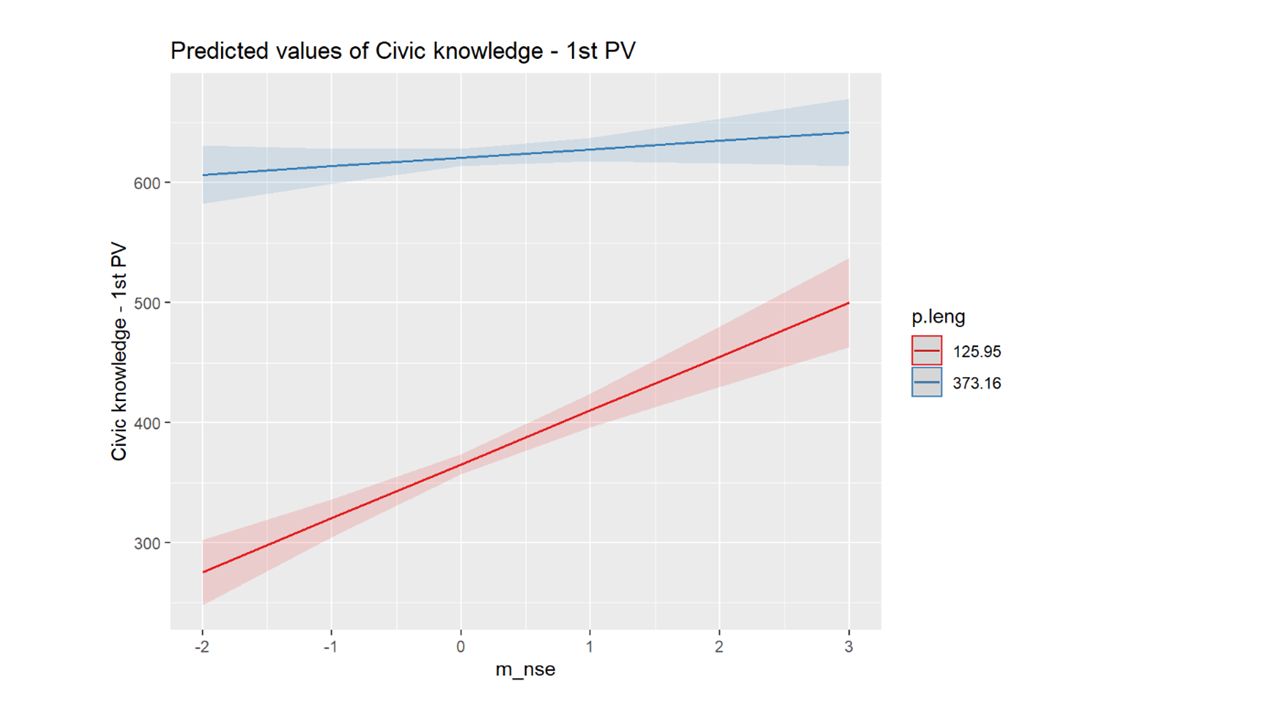
\includegraphics{../output/images/interaccionfinal.png}
\caption{La moderación de la desigualdad por el lenguaje}
\end{figure}

Como puede verse en el gráfico, la pendiente de la relación es muy
distinta si se posee un alto o un bajo nivel socioeconómico promedio de
la escuela. En escuelas con un bajo nivel socioeconómico (línea roja),
la pendiente es mucho más pronunciada y el intercepto es mucho menor.
Dicho de otra manera, en las escuelas con un nse promedio bajo, la
comprensión lectora es más determinante respecto al conocimiento cívico,
así, quienes no poseen una buena comprensión lectora siendo
establecimientos vulnerables, alcanzan 300 puntos en a la prueba de
conocimiento cívico, mientras que quienes están en una escuela con
padres de alto estatus y poseen una pésima comprensión lectora, alcanzan
450 puntos en dicha prueba. Esto, nos permite afirmar que en contextos
vulnerables es aún más importante promover el manejo del lenguaje.

Observando el gráfico anterior, llama la atención que en puntajes muy
altos de comprensión lectora, no importa el contexto económico del
colegio del estudiante. Este punto del gráfico incita a pensar que si
estudiantes de contextos vulnerables alcanzan una buena comprensión
lectora podrán desarrollar de buena manera las habilidades y
conocimientos que son necesarios para la vida ciudadana. Para evaluar
esta posibilidad, invertimos el orden del gráfico, evaluando en qué
medida un buen puntaje en el lenguaje puede moderar la relación entre
estar en un contexto escolar vulnerable y tener un deficiente
conocimiento cívico. En el gráfico 2 se evalúa dicha interacción.

En este gráfico podemos evaluar como el efecto del nivel socioeconómico
de la escuela es moderado de manera casi perfecta por la comprensión
lectora. Como puede verse, si un estudiante posee un excelente puntaje
en la prueba de comprension lectora simce, independiente del nivel
socioeconómico de su escuela, tendrá un muy alto puntaje en conocimiento
cívico. Hasta este punto, cabe la duda de si todo este efecto de la
comprensión lectora es efectivamente propio, o es más bien un reflejo de
algún efecto del colegio. Para evaluar que esto no esté ocurriendo,
replicamos el último modelo centrando la variable comprensión lectora
por el promedio de cada grupo, con el objetivo de despejar aquella
varianza que corresponde al nivel escuela. Los resultados se exponen en
la tabla número 2.

\begin{figure}
\centering
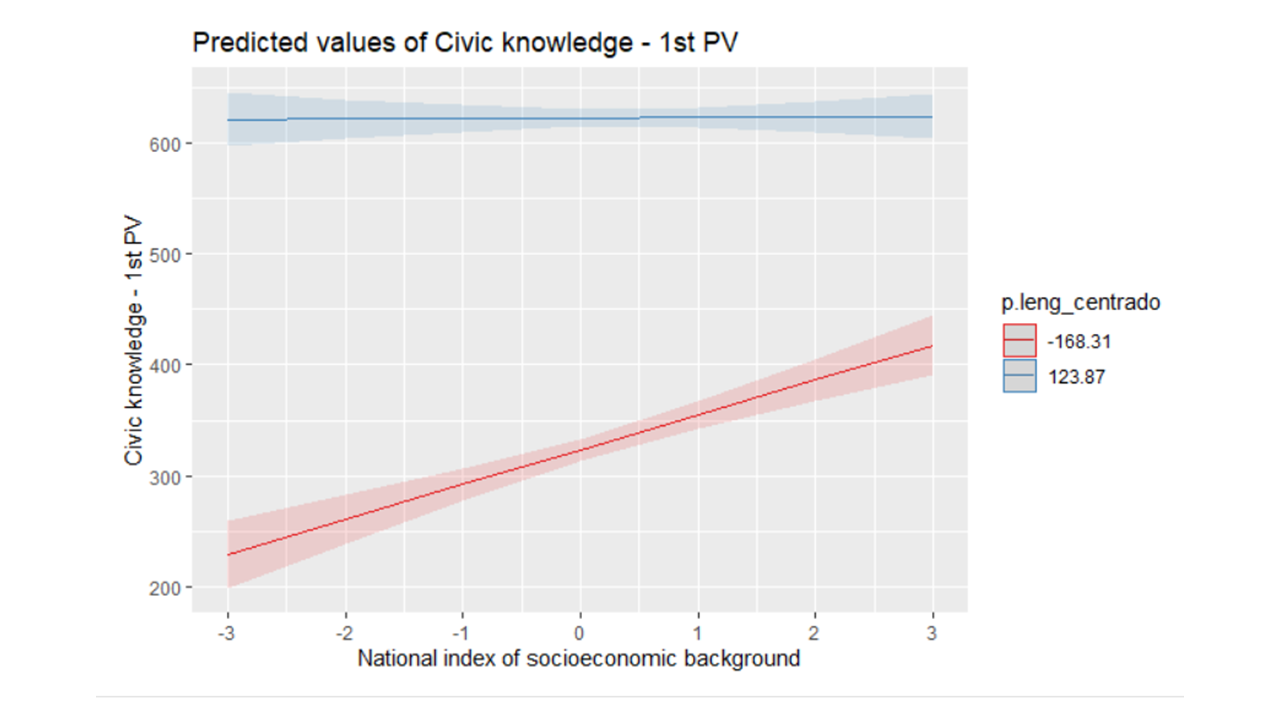
\includegraphics{../output/images/G2.png}
\caption{Evaluando el centrado}
\end{figure}

\hypertarget{conclusiones-respondiendo-las-incuxf3gnitas}{%
\section{Conclusiones: respondiendo las
incógnitas}\label{conclusiones-respondiendo-las-incuxf3gnitas}}

En consideracion de los resultados, podemos entregar algunas respuestas
parciales a nuestros objetivos de investigación.

En primer lugar, podemos decir que existe una relación moderadamente
alta entre el conocimiento Cívico y la comprensión lectora, relación la
cual no solo se mantiene al incluir otras variables fundamentales en el
modelo, sino que es capaz de controlar buena parte del efecto de las
variables de origen social. La evidencia el efecto de la comprensión
lectora, no niega el efecto positivo sobre el conocimiento Cívico que
pueden tener variables como la cultura democrática del establecimiento,
lo cual se evidencia con la mantención de este efecto al controlar por
comprensión lectora. En segundo lugar, en función de los resultados,
podemos decir que aquellas teorías que explicaban la relación entre NSE
y conocimiento cívico, por la transmisión de valores, si bien son
ciertas, poseen una visión parcial de lo que ocurre ya que en buena
medida la desigualdad social del conocimiento cívico se relaciona
ampliamente con la desigualdad social de la comprensión lectora, la cual
se relaciona con el capital cultural objetivado de los padres (más de
100 libros en el hogar) y el acceder a buena educación, lo cual se
relaciona a su vez con acceder a educación de buena calidad. Es decir,
no es tanto que los padres adinerados eduquen democráticamente a sus
hijos, sino que más bien, ya sea por transmisión directa o por acceso a
buena educación, les otorgan un mayor manejo del lenguaje, lo cual les
permite igualmente incorporar de manera más compleja la realidad
política, teniendo más herramientas para comprender, analizar y criticar
políticamente.

En tercer lugar, gracias a la evidencia, podemos señalar que la
comprensión lectora puede ser una forma de mejorar el conocimiento
Cívico en sectores vulnerables, puesto que estudiantes de dichos
sectores que si poseen un buen manejo del lenguaje poseen igualmente
altas capacidades y conocimientos para la vida ciudadana. En función de
lo anterior, se hace necesario estudiar experimentalmente el efecto que
podría tener un reforzamiento en lenguaje para la prueba de la ICCS.

\hypertarget{discusiuxf3n-las-implicancias-de-la-evidencia}{%
\section{Discusión: las implicancias de la
evidencia}\label{discusiuxf3n-las-implicancias-de-la-evidencia}}

Dados los resultados, y el rol prominente de la comprensión lectora en
el conocimiento Cívico, se hace necesario revisar algunas propuestas que
intentan explicar el conocimiento Cívico, puesto que pueden caer en
resultados espurios al no considerar una variable relevante dentro de
sus modelos.

Igualmente, se hace necesario profundizar hasta qué punto la comprensión
lectora es necesaria para vida política o más bien es un problema de
error de medida, en el cual se incorpora varianza no deseada a la
escala. En consideracion de lo anterior, es posible que, al generar
instrumentos con menores niveles de abstracción en la redacción de las
situaciones y preguntas, se generen menos de diferencias de conocimiento
Cívico entre distintos grupos sociales.

Respecto a cuáles son los caminos que deben tomarse para mejorar la
desigualdad en el conocimiento cívico y en la participación ciudadana,
resulta evidente después de los resultados, que además de reforzar la
educación cívica en los colegios como ya se está haciendo (y debe
seguirse haciendo, debe fomentarse la comprensión lectora). Incluso
podemos decir que cuando se posee altos niveles de comprensión lectora,
las diferencias de estatus socioeconómico no afectan de manera
sustancial, existiendo estudiantes de colegios con bajo nivel económico
que poseen una buena comprensión lectora y cívica. Al respecto, tipos de
clases que impliquen lectura colectiva y discusión sobre lo leído, para
entender en conjunto el sentido de los textos, puede ser una muy buena
estrategia, puesto que está demostrado que los profesores que realizan
dichas actividades mejoran el puntaje en lenguaje de sus estudiantes
(Lorena Ortega) así como que aulas más participativas poseen un efecto
para el conocimiento cívico. Es en dichos espacios de participación
donde puede sacarse el provecho al capital cultural de cada estudiante y
fomentar el efecto par.

En relación al nuevo plan de formación ciudadana, y considerando estos
resultados es sensato esperar un efecto diferencial de la política en
cada establecimiento según el nivel de comprensión lectora del colegio,
lo cual está relacionado con el nivel socioeconómico. Quizás sea
prudente en miras del objetivo de la política, prestar ayuda
especializada a colegios que posean bajos niveles de comprensión
lectora. También, dentro de los colegios prestar apoyo a los estudiantes
con dificultades al respecto también puede ser una buena medida a
aplicar en cursos anteriores al último ciclo de tercero cuarto, donde
deberán aplicar dichas habilidades en la reflexión ciudadana y en la
incorporación de conocimientos cívicos.

En tercer lugar, plantear que el conocimiento cívico está relacionado
con la comprensión lectora, levanta dudas sobre la validez del
instrumento y su capacidad de comparar países y distintos grupos
socioeconómicos. incorporar que hay estudiantes que sin conocimiento
básico logran responder preguntas de evaluación (10.1386/ctl.11.1.9\_1).

los estudiantes responden sin tener conocimiento básico llegan a altos
puntajes por lenguaje (10.1080/00933104.2012.649467)

Este punto, pone en tela de juicio la validez del instrumento, en tanto
las diferencias en comprensión lectora podrían estar inflando las
diferencias sociales en el conocimiento cívico.

Agencia de Calidad de la Educación, (2017) Estudio internacional de
Educacion Civica y Ciudadana, Presentación de resultados. Recuperado el
17 de septiembre de
\url{https://www.agenciaeducacion.cl/estudios/estudios-internacionales/iccs/}
Schulz, W., Ainely, J., Fraillon, J., Kerr, D. y Losito, B. (2011). ICCS
2009 international Report: Civic. Knowledge, attitudes, and engagement
among lower secondary school students in 38 countries. Ámstendam:
Internacional Association for the Evaluation of Educational Achievement
(IEA).

Castillo, J., Miranda D., \& Bonhomme M. (2015). Desigualdad social y
cambios en las expectativas de participación política de los estudiantes
en chile. En Cox, C. \& Castillo (Eds.).Aprendizaje de la ciudadanía
Contextos Experiencias y Resultados.

Diazgranados, S., \& Sandoval-Hernández, A. (2017). The civic competence
gaps in Chile, Colombia and México and the factors that account for the
civic knowledge gap: Evidence from the 2009

International Civic and Citizenship Education Study (ICCS). In B.
García-Cabrero, A. Sandoval-Hernández, E. TreviñoVillarreal, S.
Diazgranados Férrans, \& G. Pérez Martínez (Eds.), Civics and
citizenship: Theoretical models and experiences in Latin America.
Rotterdam, the Netherlands: Sense Publications.

Treviño, E., Béjares, C., Villalobos, C., \& Naranjo, E. (2017).
Influence of teachers and schools on students' civic outcomes in Latin
America. The Journal of Educational Research, 110(6), 604--618. doi:
10.1080/00220671.2016.1164114

Vargas-Salfate, S., Oyanedel, J. C. \& Torres-Vallejos, J. (2015).
Socialización e interés en la política en jóvenes de Chile. Revista
Latinoamericana de Ciencias Sociales, Niñez y Juventud, 13 (2),
pp.~781-794.

Bonal, X. (1998). Conflicto y reproducción en la sociología de la
educación. En: Sociología de la Educación: una aproximación crítica a
las corrientes contemporáneas (capítulo 3, pp.~71-120). Barcelona:
Paidós. ISBN: 8449305993.

Lara, B., Mizala, A. \& Repetto, A. (2010). Una Mirada a la Efectividad
de los Profesores en Chile,Revista Estudios Públicos, No 120, Centro de
Estudios Público.

Nie, N., Junn, J., Stehlik-Barry, K., (1996.) Education and Democratic
Citizenship in America. Chicago University Press, Chicago.

Kriger, M., \& Dukuen, J. (2012) Clases sociales, capital cultural y
participación política en jóvenes escolarizados una mirada desde
Bourdieu. Recuperado el 12 de septiembre en
\url{https://perio.unlp.edu.ar/ojs/index.php/question/article/view/1524/1371}

Mateos, L., Bejardo, N., Corón, A., \& López-Fernández (S.F.) Análisis
de la relación entre el interés por una materia, la creatividad y el
rendimiento académico en educación secundaria. Recuperado el 10 de
septiembre en
\url{http://www.ucm.es/BUCM/revcul/e-learning-innova/203/art3004.pdf}

Carrillo, M., Padilla, J., Rosero, T. \& Villagómez, M. (2009) La
motivación y el aprendizaje. Alteridad. Revista de Educación. Recuperado
el 13 de septiembre de
\url{https://dialnet.unirioja.es/servlet/articulo?codigo=2011378}

Lozano, L., García-Cueto, E. \& Gallo, P. (2000) Relación entre
motivación y aprendizaje. Revista Psicothema. Vol. 12, Supl. nº 2,
pp.~344-347. Recuperado el 8 de septiembre de
\url{http://www.psicothema.com/pdf/579.pdf}

Méndez Coca, D. (2015). Estudio de las motivaciones de los estudiantes
de secundaria de física y química y la influencia de las metodologías de
enseñanza en su interés. Educación XX1, 18(2), 215-235, doi:
10.5944/educXX1.14016

Schulz, W., Ainley, J., Cox, C. \& Friedman, T. (2016). Percepciones de
los jóvenes acerca del gobierno, la convivencia pacífica y la diversidad
en cinco países de América Latina. International Association for the
Evaluation of Educational Achievement (IEA).

Hoskins, B., Janmaat, J., Han, C., \&Muijs, D. (2016) Inequalities in
the education system and the reproduction of socioeconomic disparities
in voting in England, Denmark and Germany: the influence of country
context, tracking and selfefficacy on voting intentions of students age
16--18, Compare: A Journal of Comparative and International Education,
46:1, 69-92, DOI: 10.1080/03057925.2014.912796

Williams, DR y Collins, C. (1995). Diferencias socioeconómicas y
raciales en salud de los Estados Unidos: patrones y explicaciones.
Revisión anual de sociología , 21: 349-386. Valenzuela, J. (2015)
Análisis de las habilidades y dimensiones medidas en la prueba simce de
lenguaje, matemáticas y tic mediante análisis factorial. Santiago de
Chile, Agosto, 2015 Disponible en:
\url{http://146.155.94.41/handle/11534/3279/browse?type=author\&value=Valenzuela+Demarco\%2C+Jos\%C3\%A9+Miguel}.

Dukuen, Juan. (2015). Indagaciones sobre el vínculo entre política,
moral y escolaridad en la perspectiva de Bourdieu. Folios, (41),
117-128. Recuperado em 27 de junho de 2019, de
\url{http://www.scielo.org.co/scielo.php?script=sci_arttext\&pid=S0123-48702015000100008\&lng=pt\&tlng=es}.
Caro, D. H., \& Schulz, W. (2012). Ten Hypotheses about Tolerance toward
Minorities among Latin American Adolescents. Citizenship, Social and
Economics Education, 11(3), 213--234.
\url{doi:10.2304/csee.2012.11.3.213}

EcuRed (2019) Rendimiento académico. Recuperado el 20 de septiembre en
\url{https://www.ecured.cu/Rendimiento_académico} Bourdieu, P. (1979).
La Distinción: Critique Sociake du jugement. París: Les Editions de
Minuit

Burgard, S. \& Stewart, J. (2003) Occupational Status. Recuperado el 20
de septiembre en
\url{https://macses.ucsf.edu/research/socialenviron/occupation.php}
Barahona U, Planck. (2014). Factores determinantes del rendimiento
académico de los estudiantes de la Universidad de Atacama. Estudios
pedagógicos (Valdivia), 40(1), 25-39.
\url{https://dx.doi.org/10.4067/S0718-07052014000100002} MINEDUC (2019)
SIMCE. Recuperado el 20 de septiembre en
\url{https://www.agenciaeducacion.cl/evaluaciones/que-es-el-simce/}

Contreras, gonzalo, \& navia, patricio. (2013). Diferencias
generacionales en la participación electoral en chile, 1988-2010.
Revista de ciencia política (Santiago), 33(2), 419-441.
\url{Https://dx.doi.org/10.4067/s0718-090x2013000200001} Janmaat, J.G.
(2013). `Civic Competences: Some Critical Reflections' In: Print, M. and
Lange, D. (eds) Civic Education and Competences for Engaging Citizens in
Democracies. Rotterdam: Sense Publishers. pp 51-64.\\
Browne, J., Elming, W., 2015. The Effect of the Coalition's Tax and
Benefit Changes on Household Incomes and Work Incentives. Institute for
Fiscal Studies, London.

Miranda, D., Castillo, J., \& Cumsille, P. (2018). The Political
Socialization of Attitudes Toward Equal Rights from a Comparative
Perspective. En Sandoval-Hernández, A., Isac, M., \& Miranda, D. (Eds.).
Teaching Tolerance in a Globalized World (pp.~103-124). International
Association for the Evaluation of Educational Achievement (IEA).

\hypertarget{refs}{}
\leavevmode\hypertarget{ref-arendtSobreRevolucion2008b}{}%
Arendt, Hannah. 2008. \emph{Sobre La Revolución}. Buenos Aires: Alianza
Editorial.

\leavevmode\hypertarget{ref-arendtQueEsPolitica2009}{}%
---------. 2009. \emph{Qué Es La Política?} Barcelona; Bs. Aires;
México: Paidós; I.C.E. de la Universidad Autónoma de Barcelona.

\leavevmode\hypertarget{ref-arensmeierSwedishStudentsConceptual2015}{}%
Arensmeier, Cecilia. 2015. ``Swedish Students' Conceptual Knowledge
About Civics and Citizenship: An Interview Study.'' \emph{Citizenship
Teaching \& Learning} 11 (1): 9--27.
\url{https://doi.org/10.1386/ctl.11.1.9_1}.

\leavevmode\hypertarget{ref-bernsteinCLASESSOCIALESLENGUAJE1985}{}%
Bernstein, Basil. 1985. ``CLASES SOCIALES, LENGUAJE Y SOCIALIZACION.''
\emph{RCE}, no. 15 (January).
\url{https://doi.org/10.17227/01203916.5117}.

\leavevmode\hypertarget{ref-castilloSocialInequalityChanges2014}{}%
Castillo, Juan C, Daniel Miranda, Macarena Bonhomme, Cristián Cox, and
Martín Bascopé. 2014. ``Social Inequality and Changes in Students'
Expected Political Participation in Chile.'' \emph{Education,
Citizenship and Social} 9 (2): 140--56.
\url{https://doi.org/10.1177/1746197914520650}.

\leavevmode\hypertarget{ref-contrerasDIFERENCIASGENERACIONALESPARTICIPACION2013}{}%
Contreras, Gonzalo, and Patricio Navia. 2013. ``DIFERENCIAS
GENERACIONALES EN LA PARTICIPACIÓN ELECTORAL EN CHILE, 1988-2010.''
\emph{Rev. Cienc. Polít. (Santiago)} 33 (2): 419--41.
\url{https://doi.org/10.4067/S0718-090X2013000200001}.

\leavevmode\hypertarget{ref-coxAprendizajeCiudadaniaContextos2015}{}%
Cox, Cristián, and Juan Carlos Castillo, eds. 2015. \emph{Aprendizaje de
La Ciudadanía: Contextos, Experiencias Y Resultados}. Santiago:
Ediciones Universidad Católica de Chile.

\leavevmode\hypertarget{ref-elmingEffectCoalitionTax2015}{}%
Elming, William, and James Browne. 2015. ``The Effect of the Coalition's
Tax and Benefit Changes on Household Incomes and Work Incentives.''
Institute for Fiscal Studies.
\url{https://doi.org/10.1920/BN.IFS.2015.00159}.

\leavevmode\hypertarget{ref-EstudioInternacionalEducacion2017}{}%
``Estudio Internacional de Educacion Civica Y Ciudadana, Presentación de
Resultados. Agenciaeducacion.'' 2017. 2017.
\url{https://www.agenciaeducacion.cl/estudios/estudios-internacionales/iccs/}.

\leavevmode\hypertarget{ref-ferransCivicCompetenceGaps2017}{}%
Ferráns, Silvia Diazgranados, and Andrés Sandoval-Hernández. 2017. ``The
Civic Competence Gaps in Chile, Colombia and Mexico and the Factors That
Account for the Civic Knowledge Gap.'' In \emph{Civics and Citizenship},
edited by Benilde García-Cabrero, Andrés Sandoval-Hernández, Ernesto
Treviño-Villareal, Silvia Diazgranados Ferráns, and María Guadalupe
Pérez Martínez, 155--92. Rotterdam: SensePublishers.
\url{https://doi.org/10.1007/978-94-6351-068-4_8}.

\leavevmode\hypertarget{ref-janmaatCivicCompetences2013}{}%
Janmaat, Jan Germen. 2013. ``Civic Competences.'' In \emph{Civic
Education and Competences for Engaging Citizens in Democracies}, edited
by Murray Print and Dirk Lange, 51--63. Rotterdam: SensePublishers.
\url{https://doi.org/10.1007/978-94-6209-172-6_5}.

\leavevmode\hypertarget{ref-joignantDesigualdadesVozPolitica2017}{}%
Joignant, Alfredo, Matías Bargsted, Nicolas Somma, and Tomás Campos.
2017. ``Desigualdades de Voz Política En Chile.''
\url{https://doi.org/10.13140/RG.2.2.28798.28480}.

\leavevmode\hypertarget{ref-lechnerConflictivaNuncaAcabada1984}{}%
Lechner, Norbert. 1984. \emph{La Conflictiva Y Nunca Acabada
Construcción Del Orden Deseado}. Serie Libros FLACSO-Chile 10. Santiago,
Chile: Facultad Latinoamericana de Ciencias Sociales.

\leavevmode\hypertarget{ref-mirandaDesigualdadCiudadaniaAproximacion2018}{}%
Miranda, Daniel. 2018. ``Desigualdad Y Ciudadanía : Una Aproximación
Intergeneracional.'' Tesis Doctoral, Santiago: Pontificia Universidad
Católica de Chile. \url{https://repositorio.uc.cl/handle/11534/22255}.

\leavevmode\hypertarget{ref-schlozmanUnequalUnrepresentedPolitical2018}{}%
Schlozman, Kay Lehman. 2018. \emph{Unequal and Unrepresented: Political
Inequality and the People's Voice in the New Gilded Age}. Princeton:
Princeton University Press.

\leavevmode\hypertarget{ref-Schlozman1999}{}%
Schlozman, Kay, Sidney Verba, and Henry Brady. 1999. ``Civic
Participation and the Equality Problem.'' In, 427--59.

\leavevmode\hypertarget{ref-schmittConceptoPoliticoTexto1998}{}%
Schmitt, Carl. 1998. \emph{El Concepto de Lo Político Texto de 1932 Con
Un Prólogo Y Tres Corolarios}. Madrid (España): Alianza.

\leavevmode\hypertarget{ref-informeiccs2011}{}%
Schulz, Wolfram, John Ainley, Julian Fraillon, David Kerr, and Bruno
Losito. 2010. ``ICCS 2009 International Report: Civic Knowledge,
Attitudes, and Engagement Among Lower- Secondary School Students in 38
Countries,'' January.

\leavevmode\hypertarget{ref-trevinoInfluenceTeachersSchools2017}{}%
Treviño, Ernesto, Consuelo Béjares, Cristóbal Villalobos, and Eloísa
Naranjo. 2017. ``Influence of Teachers and Schools on Students' Civic
Outcomes in Latin America.'' \emph{The Journal of Educational Research}
110 (6): 604--18. \url{https://doi.org/10.1080/00220671.2016.1164114}.

\leavevmode\hypertarget{ref-zhangUnderstandingCivicCognitive2015}{}%
Zhang, Ting, Judith Torney-Purta, and Robert J. Mislevy. 2015.
``Understanding Civic Cognitive Assessment Tasks: Associations Between
Linguistic Features and Students' Task Performance.'' \emph{Citizenship
Teaching \& Learning} 11 (1): 29--47.
\url{https://doi.org/10.1386/ctl.11.1.29_1}.

\end{document}
